\chapter{Paper 3}\label{sc:p3}
\textbf{\Large Resonators In Open-Loop Sigma-Delta Modulators}\\
\indent Carsten Wulff and Trond Ytterdal\\
\indent Submitted to IEEE Transactions on Circuits and Systems I: Regular papers\\
%\def\abstract{\section{Abstract}}
\renewcommand\myfigname{sdrfig:}
\renewcommand\myeqname{sdreq:}
%\renewcommand{\appendices}{}
%\newcommand{\myappname}{Section}
\newcommand{\myappname}{Section }
\newcommand{\myappendices}{}

%\newcommand{\myintmodref}{}
\newcommand{\mymodintfig}{
 \begin{figure}[htbp]
   \centering{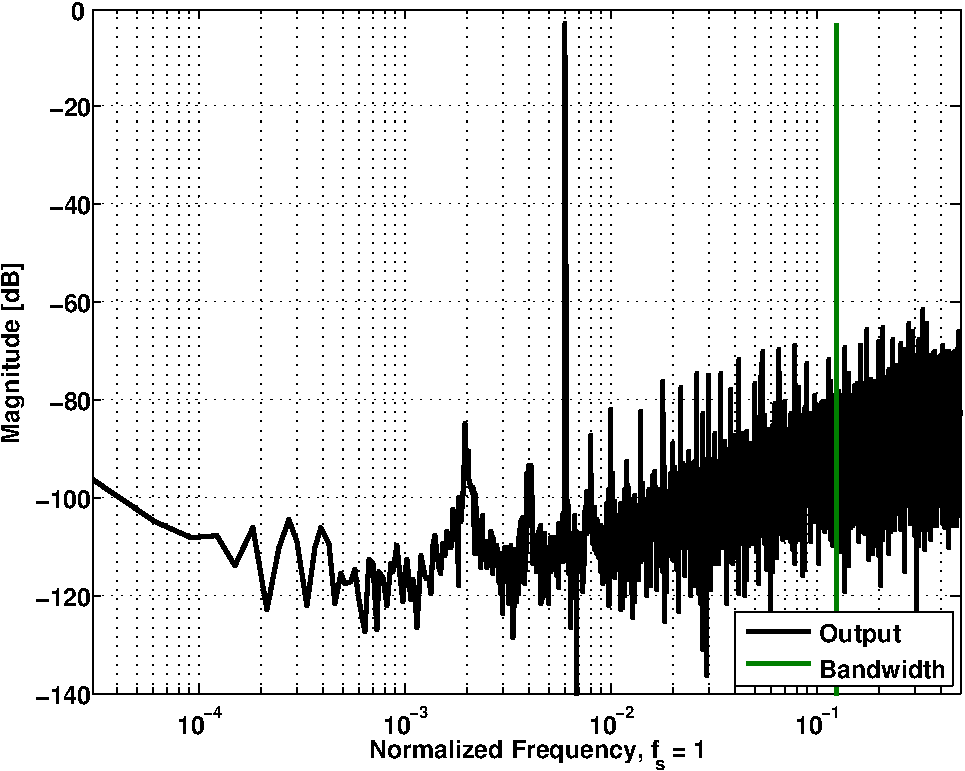
\includegraphics[width=\myfigwidth]{graphics/intmod_z}}
   \caption{SIMULINK model, SNDR = 52.20-dB}
   \label{sdrfig:intmod_z} 
 \end{figure}

 \begin{figure}[htbp]
   \centering{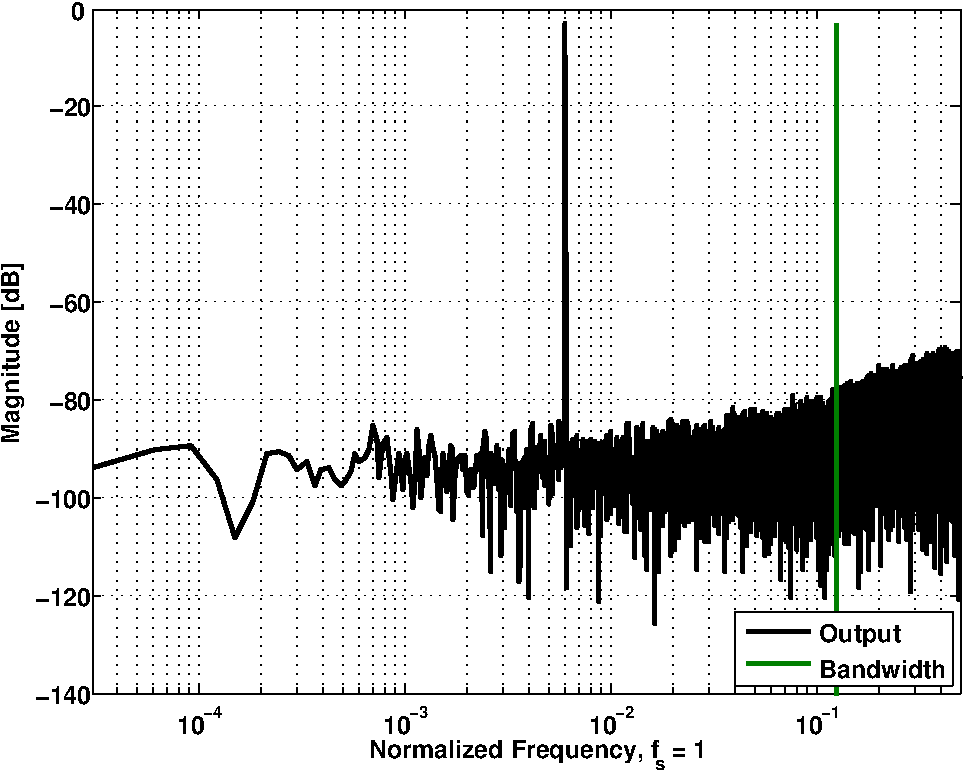
\includegraphics[width=\myfigwidth]{graphics/intmod_d}}
\caption{Approximation, SNDR = 51.44-dB}
\label{sdrfig:intmod_d}
\end{figure}

\begin{figure}[htbp]
\centering{ 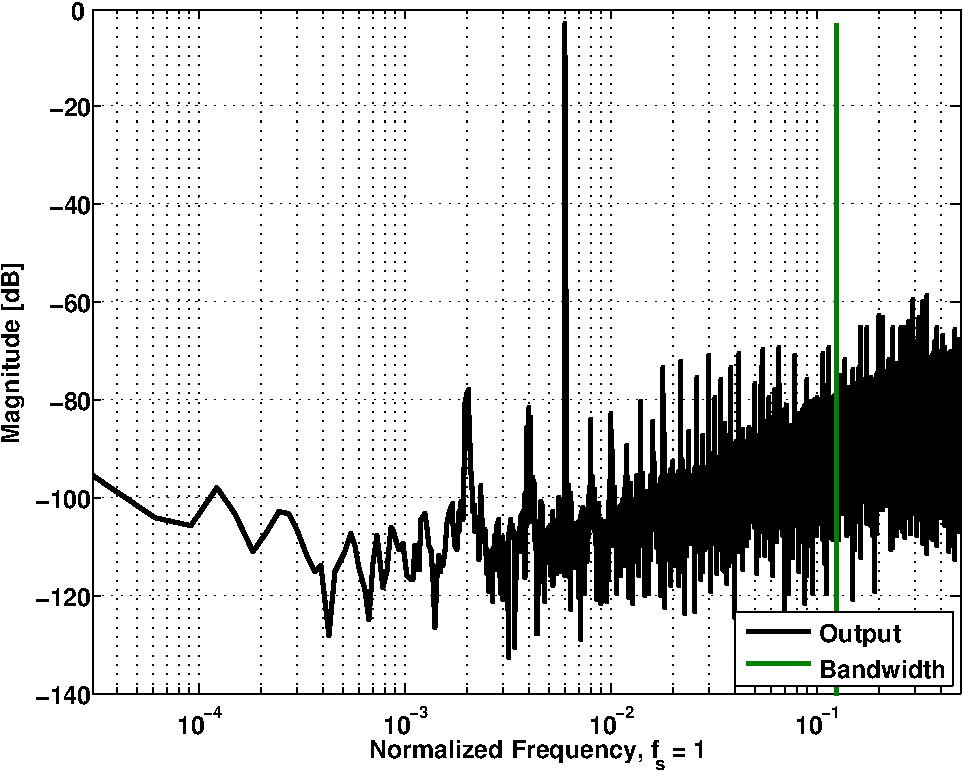
\includegraphics[width=\myfigwidth]{graphics/intmod_spice}}
\caption{SPICE model, SNDR = 51.66-dB}
\label{sdrfig:intmod_spice}
\end{figure}

\begin{figure}[htbp]
\centering{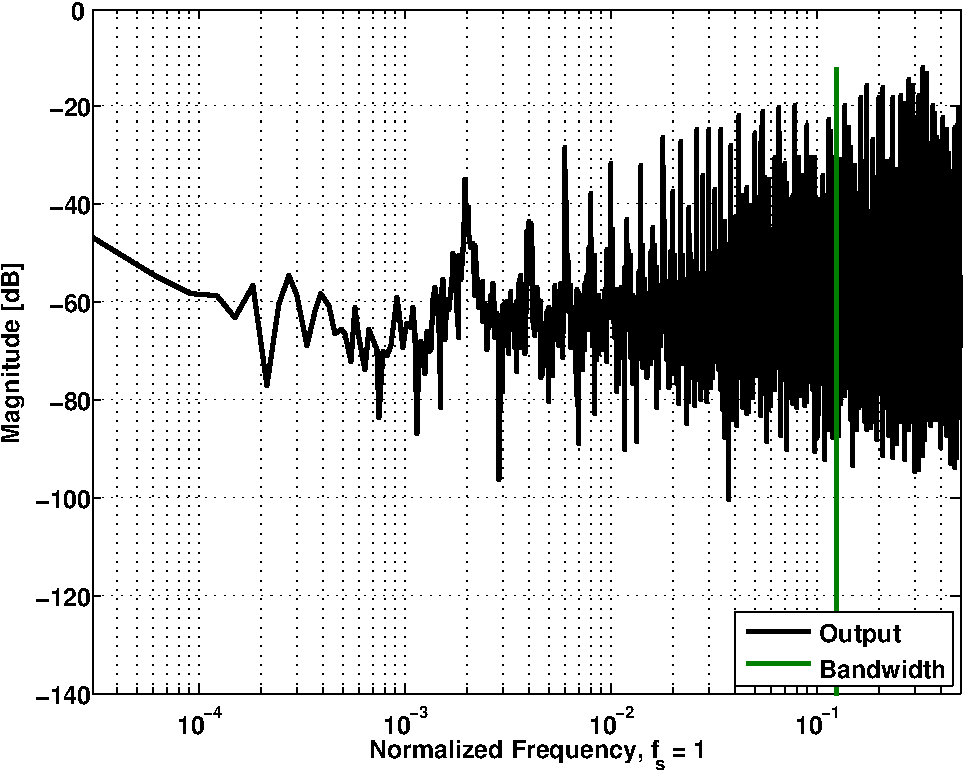
\includegraphics[width=\myfigwidth]{graphics/intmod_u}}
 \caption{FFT of $u_n$}
\label{sdrfig:intmod_u} 
\end{figure}

}

\section*{Errata}
We recieved a response to this paper quite quickly, and all
reviewers found the paper interesting, but wanted more information. We
were asked to submit a new version for review with the following
changes. 
\begin{itemize}
\item Discuss the effects of mismatch in capacitors
\item Discuss why adding zeros at non-zero frequency is better than at
  zero frequency
\item Add more introduction to OLSDM and SDM
\item Discuss the effects of offset errors in comparators
\end{itemize}
These changes have been included in the paper below.




\newcommand{\simulink}{Simulink  }
\newcommand{\matlab}{MATLAB }
%\CWabstract{
%\section*{Abstract}
%########################################################################
%\begin{quote}
%{\center\textbf{Abstract:}}\\
\begin{abstract}
In this paper we introduce the modulo resonator for use in \textit{open-loop
sigma-delta modulators} (OLSDM). The OLSDM presented in this work is
intended for use in high accuracy (14-bit), high-speed analog-to-digital
converters.

The modulo resonator is used with a modulo notch filter to
insert a zero in the noise transfer function at a non-zero
frequency. 
The effect of finite gain in modulo integrators and modulo resonators
are described and verified through simulation. 
The modulo resonator and previously published modulo
integrator are used in a behavioral model of a switched-capacitor fifth-order OLSDM with more
than 13-bit effective number of bits for an oversampling ratio of
four. We prove for
the N-order OLSDM that the number of bits in the quantizer (B) must be
larger than N to ensure equivalence between OLSDM and sigma-delta
modulation.
\end{abstract}
%\end{quote}
%}

\begin{keywords}
%\keywords{ 
Sigma-delta modulators, switched-capacitor circuits, modulo
integrator, modulo resonator, open-loop sigma-delta modulators
\end{keywords}

%########################################################################
\section{Introduction}
%########################################################################
If one wants to make an analog-to-digital converter with high
resolution ($>$12-bit) a sigma-delta modulator is a natural choice. 
Sigma-delta modulators are prevalent as analog-to-digital converters in applications with low to medium
bandwidth  ($<$ 10MS/s) and high resolution.  
The sigma-delta modulator trades speed for resolution.
It typically uses a low-resolution quantizer ($<$
6-bit) with a large quantization error. The quantizer is run at a
higher speed than required by the system bandwidth. By using clever
analog-filters and feedback techniques the in-band quantization error can be
lowered, while the out-of-band quantization error can be large. This
out-of-band quantization error is easily filtered using digital
filters. 

The family of sigma-delta modulators is large, with
many diverse family members. One of the oldest members is the low-pass
sigma-delta modulator, which in its simplest form consists of an
integrator followed by a quantizer. The quantized signal is fed-back
to the input through a digital-to-analog converter (DAC) and subtracted from
the input. The transfer function of the modulator is different for the
input signal and the quantization noise.\footnote{This assumes a linear model of the quantizer,
  since the transfer function is only defined for a linear system} The input
signal will undergo an integration followed by a
differentiation and have a transfer function of one. The quantization noise will be
differentiated and thus high pass filtered. 

In an ideal world, with no voltage swing limitations, a low-pass
sigma-delta modulator
could be implemented by an integrator 
followed by a quantizer and a differentiator, but since supply voltage
is limited in electronic circuits, and an integrator  
has infinite DC gain, it is difficult to implement. Somehow
the output swing of the integrator has to be limited. Feedback is
typically used to limit the output swing of the integrator. 
 
In this
paper we discuss a small sub group that we denote Open-loop sigma-delta
modulators (OLSDM).  We define OLSDM as \textit{any sigma-delta modulator that does
not have feedback of the quantized modulator output signal}. 

The idea of a open-loop sigma-delta modulator is to use a limiting
function (for example a modulo) to limit the signal swing in the
analog domain, replacing the feedback of the quantized signal. After
quantization  the inverse limiting function is used to reverse the
effects of the limit in the analog domain. This idea is
by no means new. One of the first suggestion of an OLSDM was almost thirty years ago in
\cite{claasen80}. Although there was no system 
implementation they explained a method that avoided feedback of the
quantized signal. Little over a decade ago the  Frequency
Sigma-Delta Modulator (FSDM) \cite{hovin97.2} was presented, and more
recently \cite{wismar07a}. 
In the FSDM a voltage controlled
oscillator (VCO) is used as the modulo integrator, and it was shown in \cite{hovin97.2} that the pre-processing
in FSDM is equivalent to modulo integration. 
The
non-feedback \SD digital-to-analog modulator, where the
integrator is implemented as a digital modulo integrator, was
described in \cite{wisland03a}. 
In \cite{wulff08a} an amplitude modulated switched-capacitor open-loop
sigma-delta modulator was introduced. A switched-capacitor 
modulo integrator was used to perform the modulo integration.

An example of analog-to-digital conversion with open-loop sigma-delta
modulation is shown in Fig.
\ref{sdrfig:olsdm-basic}. The input
signal, $x$, is accumulated by the integrator ($\langle\Sigma\rangle$). The
integrator in Fig. \ref{sdrfig:olsdm-basic} is a modulo integrator that
wraps around when the sum exceeds the
range ($R$). The output of the integrator ($u$) is quantized by a quantizer,
which is modeled as a linear addition of
quantization noise ($q$). The conditions  for modeling a
quantizer as linear addition of noise was covered in 
\cite{widrow56}. The modulo differentiator ($\langle\Delta\rangle$) reverse the effect
of the modulo
integrator. The decimation filter required to down-sample the output of
the modulator is not shown. 

In this modulator the input signal passes through unchanged. The quantization noise pass through the
differentiator and is first order high-pass filtered. 

The sigma-delta modulator in Fig. \ref{sdrfig:olsdm-basic} is equivalent
to a first order
low-pass sigma-delta modulator providing certain conditions are met.

\begin{figure}[htbp]
\centerline{ 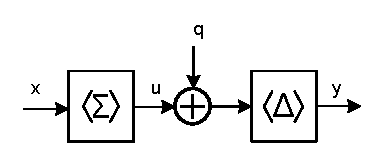
\includegraphics[width=\myfigwidthb]{graphics/osd}}
  \caption{First order low-pass open-loop sigma-delta modulator}
  \label{sdrfig:olsdm-basic}
\end{figure}

The application envisioned for the  OLSDM discussed in this paper is as a front-end in a high
speed ($>$10MS/s), high resolution (14-bit)  analog-to-digital converter. The advantage of OLSDM is that
it is trivial to use high-latency quantizers since there is no feedback of the quantized
modulator output. 

There are two unsolved challenges that this paper discuss: when is
open-loop sigma delta modulation equivalent to sigma-delta modulation,
and how to introduce zeros in the noise transfer function (NTF) at non-zero
frequencies. 

%-------------------------------------------------------
\subsection{When is OLSDM equivalent to SDM?}
%-------------------------------------------------------
It is observed in simulation that open-loop sigma-delta
modulation (OLSDM) is not always equal to
sigma-delta modulation (SDM). Whether an OLSDM works as an SDM depends
on the input signal amplitude and the number of bits in the
quantizer. The input signal amplitude must be less than $|x_n| < R/2$
(0dBFS\footnote{0dB referred to full scale amplitude, $R/2$}), but OLSDM sometimes
loose its noise shaping at less than 0dBFS. 

In \cite{wulff08a} an error
correction scheme was used to restore the noise shaping for input
signal amplitudes up to 0dBFS. But the error correction assumed that
the input frequency was much less than the sampling frequency ($f_i << f_s$). For some applications (like high speed, high
resolution) the OSR can be low ($OSR < 8$) and $f_i << f_s$ is no
longer valid. 

The number of bits in the quantizer affect the equivalence
between OLSDM and SDM. It is observed that the number of bits in
the quantizer must be larger than the order of the modulator. This was
proved for the special case of a second order OLSDM in
\cite{wisland02a}.

We will prove for
the N-order OLSDM that the number of bits in the quantizer (B) must be
larger than the order (N) to ensure equivalence between OLSDM and SDM.

\subsection{Zeros in NTF at non-zero frequency}
Previous OLSDMs have all been low order low-pass sigma-delta
modulators. Low order low-pass sigma-delta modulators are unsuited for high
conversion rate applications due to the high oversampling ratio
required to get high resolution, assuming a low resolution quantizer
is used. 

If the sampling frequency ($f_s$) is constant, the resolution can be increased by
adding more zeros to the noise transfer function (NTF). Adding zeros at a non-zero
frequency ($\omega_0 > 0$) reduce the OSR more than adding them at
zero frequency. To see why zeros at a non-zero frequency reduce the
OSR more than adding them at zero frequency it is instructive to look at a
graphical comparison. In \reg{f0zerof1} a comparison between two
fifth-order sigma-delta modulators is shown, one with all zeros at
zero-frequency (dashed line) and one modulator with one zero at
zero-frequency and two complex conjugate zeros at non-zero frequencies
(solid line). Since the noise
transfer function is real the zeros must be complex conjugate, thus to
get two zeros at non-zero frequency we need four zeros, two at
positive frequencies and two at negative frequencies. The dominating
contribution from the noise transfer functions will be at high
frequencies. So although the NTF with non-zero frequency zeros has less
attenuation at low frequencies it has more attenuation at high
frequencies (for example at a normalized frequency of 0.1 the
difference is almost 20dB). Accordingly, for an oversampling ratio of
four (marked by the dotted line), the NTF with zeros at a non-zero
frequency has more attenuation, and as a consequence yields a higher
resolution for a given OSR.

\begin{figure}[htbp]
\centerline{ 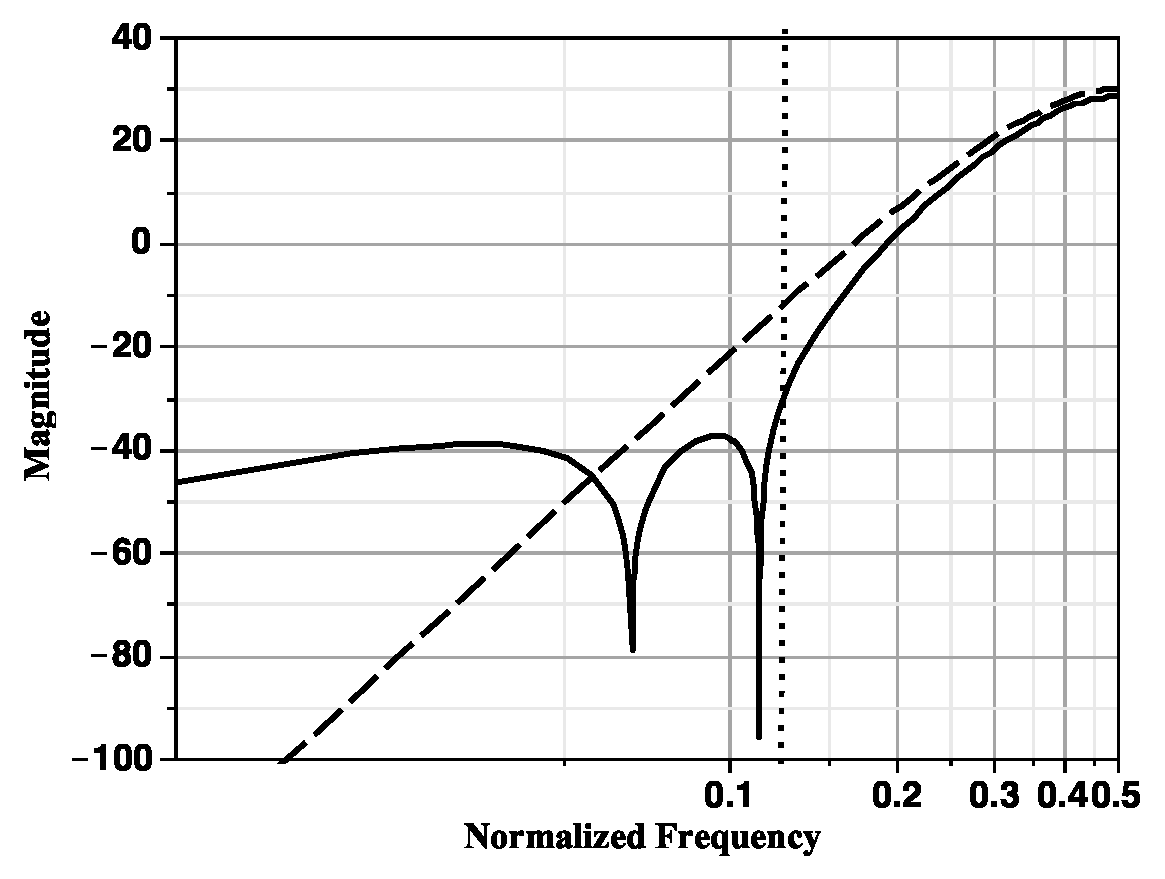
\includegraphics[width=\myfigwidth]{graphics/f0zerof1}}
  \caption{Comparison between a fifth-order sigma-delta modulator with
  all zeros at zero frequency (dashed-line) and fifth-order
  sigma-delta modulator with one zero at zero
  frequency and two complex conjugate zeros at optimum frequencies.}
  \label{sdrfig:f0zerof1}
\end{figure}


To the best of our
knowledge, zeros at non-zero frequencies have not been used in OLSDM
before this work. 

The paper is organized as follows: In Section \ref{sdrbasicmodulo} 
OLSDM is explained and requirements for input signal amplitude and quantizer bits are
derived. In Section \ref{sdrmodulointegrators} the key component of OLSDM, the
modulo integrator, is described in detail, including the effects of
finite gain in modulo integrators. The modulo integrator has
previously been described in \cite{wulff08a}, but the effects of
finite gain in modulo integrators has not been exhaustively covered.

The modulo resonator is introduced in
Section \ref{sdrmoduloresonator}. The modulo integrator and modulo
resonator are combined in Section \ref{sdrmatlabsim} to make a behavioral
model of a fifth
order low-pass OLSDM with more than 13-bit effective number of bits with an
OSR of four. Simulation results from behavioral level models in \matlab \cite{matlab}
and SPICE are presented in Section \ref{sdrmatlabsim}.


%########################################################################
\section{When is OLSDM equivalent to SDM?}\label{sdrbasicmodulo}
%########################################################################
The modulo operator is used extensively in OLSDM to limit the signal
swing at the output of modulo integrator. The modulo operator is written as
\eqn{
\label{sdreq:modulo}
  x_r = \langle x \rangle_R
}
where $x \in \langle -\infty,\infty \rangle $ is the input signal, $R$ is the range and
$x_r  \in \langle - R/2, R/2 \rangle$ is the residue after dividing by
the range, $R$. 
This
modulo function is not the normal mathematical modulo function, but
a
function that computes the remainder of the input signal after
rounding it to an integer number of full scale signal swings ($R$).

The modulo is similar 
to what was used in \cite{lipshitz07} where they proved the
equivalence of the  open-loop and closed loop representations by
symbolic manipulation. The modulo arithmetic used in OLSDM has  previously been used in
comb filters, as was
shown in \cite{chu84}. 
%The discrete time equations for OLSDM will be derived, and from
%these it will be shown that a open-loop sigma-delta modulator is equivalent
%to a sigma-delta modulator, provided certain conditions of the input signal amplitude
%and the quantizer bits are met.

The following theorem is useful for the derivations below.
\begin{theorem}
The modulo of the sum of modulo is equal to the modulo of sum if the range of the
two modulus are equal, $R_0 = R_1=R$
\eqn{
\label{sdreq:prop1}
\langle \langle x \rangle_{R_0} + \langle y \rangle_{R_0} \rangle_{R_1} = \langle
  x + y \rangle_R
}
\end{theorem}
A proof of the theorem is included in \myappname \ref{sdrap:modproof}

The modulo integration, shown in Fig \ref{sdrfig:olsdm-basic}, is
written as
\eqn{
\label{sdreq:modint}
  u_n = \left\langle\sum_{i=0}^\infty{x_{n-i-1}}\right\rangle_R
}
where $x_n$ is the input signal to the integrator at time $n$, $u_n$ is the
modulator output signal, and $n$ is the discrete time step. The input signal at
time $n-1$ is written as $x_{n-1}$.

The output of the modulator in Fig. \ref{sdrfig:olsdm-basic}
is
\eqn{
\label{sdreq:modout}
  y_n = \left\langle u_n - u_{n-1} + q_n - q_{n-1}\right\rangle_R
}
where $q_n$ is the quantization noise. 

Insert \req{modint} in
\req{modout} and let $e_n = q_n - q_{n-1}$

\eqn{
\label{sdreq:modout1}
  y_n = \left\langle \left
      \langle\sum_{i=0}^\infty{x_{n-i-1}}\right\rangle_R -
    \left\langle\sum_{i=0}^\infty{x_{n-i-2}}\right\rangle_R  + e_n \right\rangle_R
}
With \req{prop1}  \req{modout1} reduces to
\eqn{ 
\label{sdreq:modout3}
  y_n = \left\langle x_{n-1} + e_n \right\rangle_R
}
The discrete time equation for a first order low-pass sigma-delta
modulator is
\eqn{
\label{sdreq:sdm}
  y_n  = x_{n-1} + q_n - q_{n-1}
}
Equation \req{modout3} is equal to \req{sdm} if 
\eqn{
  | x_n  + e_n| < R/2
}

The absolute value of the filtered quantization noise ($|e_n|$) has a
maximum value of one LSB (Least
Significant Bit), since $|q_n| \leq 1/2 LSB$ and $e_n = q_n -
q_{n-1}$. Here $LSB = R/2^B$, where $B$ is the number of 
bits in the quantizer. 

The input signal for first order open-loop
sigma-delta modulator must be limited by 
\eqn{
\label{sdreq:modlimit}
  |x_n| < R/2 - 1 LSB = R( 1/2 -1/2^B)
}
%Equation \req{modlimit} clearly shows that quantizers with few bits
%are unsuited for OLSDM, since they would place severe limitations on
%the input signal. 
We will derive the general input signal limitations for N-order OLSDM,
but to reduce the length of equations we define
\eqn{
  f_{x,n} = \sum_{i=0}^\infty{x_{n-i}}
}
and from \req{prop1}
\eqn{
\label{sdreq:fdef1}
  \left\langle \langle f_{x,n} \rangle_R  - \langle f_{x,n-1} \rangle_R
  + e_n \right \rangle_R = \langle x_n +e_n \rangle_R
}

For second order OLSDM (Fig. \ref{sdrfig:mod2}) the
output of the first integrator is
\eqn{
  u_n = \langle f_{x,n-1} \rangle_R      
}
and the output of the second integrator is
\eqn{
  u_{1,n} = \langle f_{u,n-1} \rangle_R
}

\begin{figure}[htbp]
\centerline{ 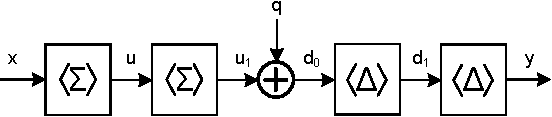
\includegraphics[width=\myfigwidth]{graphics/osd2}}
  \caption{Second order low-pass open-loop sigma-delta modulator}
  \label{sdrfig:mod2}
\end{figure}

The quantized signal is 
\eqn{
  d_{0,n} = \langle f_{u,n-1} \rangle_R + q_n
}
And the output signal of the first modulo differentiator is
\eqn{
  d_{1,n} = \left\langle \langle f_{u,n-1} \rangle_R - \langle f_{u,n-2}
    \rangle_R +e_n\right\rangle_R
}
which by \req{fdef1} is written as
\eqn{
  d_{1,n} = \langle u_{n-1} + e_n \rangle_R
}
The output signal of the modulator is
\eqn{
y_n = \left \langle \langle f_{x,n-1} \rangle_R - \langle f_{x,n-2}
  \rangle_R + e_n - e_{n-1} \right\rangle_R
}
which by \req{fdef1} is
\eqn{
\label{sdreq:modout2}
y_n = \left \langle x_{n-1}  + q_n - 2 q_{n-1} + q_{n-2} \right\rangle_R
}

The maximum absolute
value of the quantization noise in 
\req{modout2} is 
\eqn{|q_n| + |2q_{n-1}| + |q_{n-2}| = 1/2 + 1 +1/2 =
2
}
From this it follows that the input signal must be limited by
\eqn{
\label{sdreq:lim2}
  |x_n| < R/2 - 2 LSB = R(1/2 - 2/2^B)
}
\req{lim2} is sufficient to ensure that the second order
OLSDM is equivalent to a second order SDM. It can be shown that for third
order OLSDM the requirement is  
\eqn{
  |x_n| < R/2 - 4 LSB = R(1/2 - 4/2^B)
}
For N-order OLSDM the input signal must be limited by
\eqn{
\label{sdreq:inlimit}
  |x_n| < R(1/2 - 2^{N-1}/2^B)
}
If $B=N$ the input signal limit is not practical since
\eqn{
  |x_n| < R(1/2 - 2^{N-1}/2^B) = R(1/2-1/2) = 0
}
Accordingly, $B > N$ to ensure that N-order OLSDM is equivalent to
N-order SDM. This is equivalent to the quantizer 
non-overload criteria in SDM proved in
\cite{lokken06}. An N-order sigma-delta modulator will not overload
the quantizer if the input signal is limited by
$|x_n| < R/4$, and $B=N+1$. 

For $B=N+1$ in \req{inlimit}
\eqn{
  |x_n| < R(1/2 - 1/4) = R/4
}

In the next section we will cover the key component of
analog-to-digital OLSDM, the modulo integrator.



%########################################################################
\section{Modulo integrator}\label{sdrmodulointegrators}
%########################################################################

In this section we discuss the implementation of a
modulo integrator in behavioral level models, the switched-capacitor
implementation, and effects of finite opamp gain in the modulo integrator. 

%-------------------------------------------------------
\subsection{Behavior level implementation}
%-------------------------------------------------------
The output of the modulo integrator is described by 
\eqn{
\label{sdreq:modint_copy}
  u_n = \left\langle\sum_{i=0}^\infty{x_{n-i-1}}\right\rangle_R
}
In behavioral level models \req{modint_copy} is impractical 
due to the infinite modulo. In the definition of the
modulo \req{modulo}  the input signal can take any value,
$x_n \in \langle-\infty,\infty\rangle$. This requires the modulo
integrator to wrap around infinitely many times if the output signal
is to be limited by $u_n \in \langle -R/2, R/2\rangle$. But since the
input signal is limited by \req{inlimit}, the infinite modulo is
unnecessary. Assume that $|x_n| < R/2$, which by
\req{inlimit} must be true, then the maximum value after integration
,but before the modulo, is limited by $u_{before,n} \in \langle -R, R
\rangle$. Fig. \ref{sdrfig:modint} shows an example of the output
($u_{before,n}$) before modulo, and after modulo ($u_n$) for a sinusoidal
input signal ($x_n$). The modulo integrator is implemented by adding or
subtracting the range $R$.
\begin{figure}[htbp]
\centerline{ 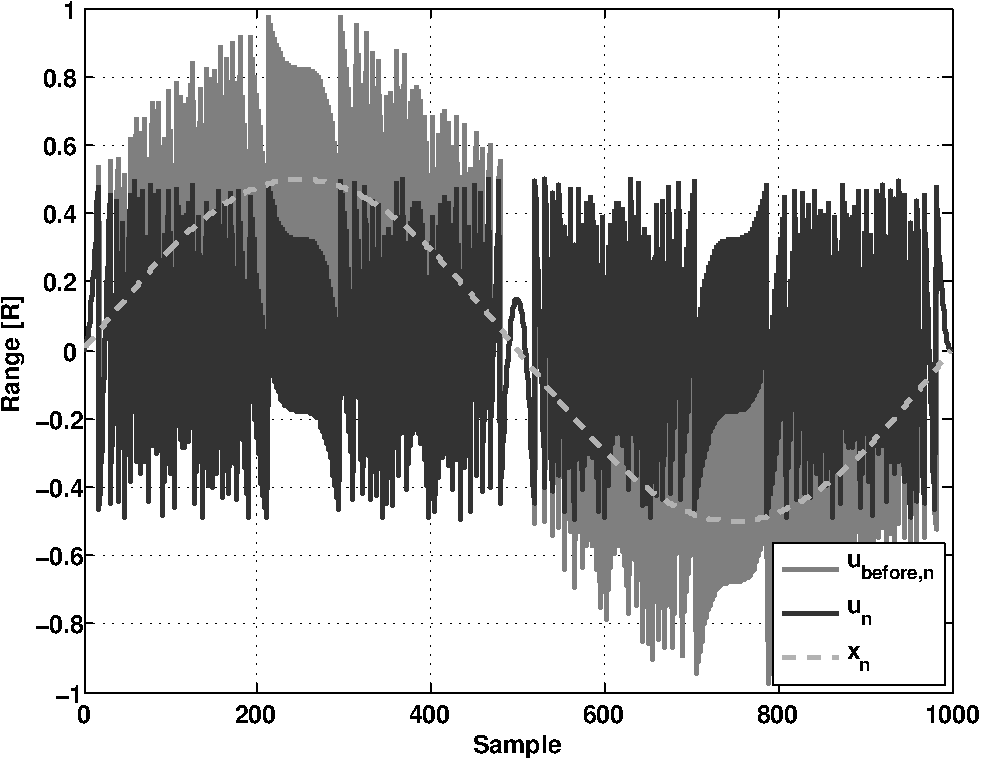
\includegraphics[width=\myfigwidth]{graphics/modint_res}}
  \caption{States of the modulo integrator for a sinusoidal input
    $x_n$. The output before modulo is $u_{before,n}$ and the output
    after is $u_n$.}
  \label{sdrfig:modint}
\end{figure}
The modulo operation can now be defined as
\eqn{
  u_{before,n} = u_{n-1} + x_{n-1}
}
and 
\begin{numcases}{u_n = }
\label{sdreq:modintdef}
u_{before,n} + R & $u_{before,n} \in \langle -R, -R/2 ]$\nonumber\\ 
u_{before,n}  & $u_{before,n} \in \langle -R/2 , R/2 \rangle$ \nonumber\\
u_{before,n} - R & $u_{before,n} \in [ R/2, R \rangle$
\end{numcases}
%or written as \req{modulo}
%\eqn{
%\label{sdreq:limmodulo}
%  x_r = \langle x \rangle_R,\: x \in \langle -R,R  \rangle, \: x_r \in
%  \langle -R/2,R/2 \rangle
%}


The modulo integrator described by \req{modintdef} can be implemented
as a switched-capacitor (SC) circuit \cite{wulff08a}. 

%-------------------------------------------------------
\subsection{Switched-capacitor modulo integrator}\label{sdrSscmod}
%-------------------------------------------------------
The SC modulo integrator is based on the
parasitic insensitive integrator shown in Fig. \ref{sdrfig:scint}. The
input signal is sampled at the end of $p_1$. In $p_2$ the charge of
$C_1$ is moved to $C_2$ by forcing node $V_x$ equal to zero
with the opamp.
\begin{figure}[htbp]
\centerline{ 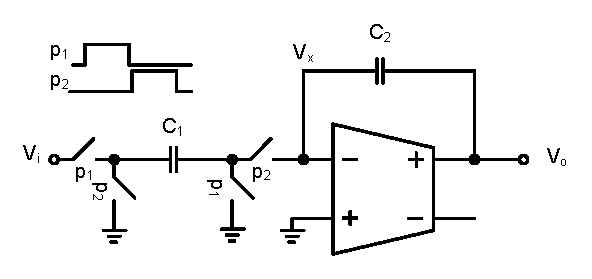
\includegraphics[width=\myfigwidth]{graphics/sc_int}}
  \caption{Parasitic insensitive switched-capacitor integrator}
  \label{sdrfig:scint}
\end{figure}
The switched-capacitor modulo integrator is shown in
Fig. \ref{sdrfig:scmod}. Three
clock phases are needed for the modulo integrator, $p_1$, $p_2$, and
$p_3$. The clock period is divided into four equally large phases
$t_0$, $t_1$, $t_2$, $t_3$ for a
straightforward implementation. Phase one is the combination of
the first two phases ($p_1 = t_0 + t_1$), phase two is the
combination of the last two phases ($p_2 = t_2 + t_3$), and phase three is
equal to the last phase ($p_3= t_3$). 

The input signal $V_{i}$ is
sampled across capacitor $C_1$ during $p_1$. In $p_2$ the charge
across $C_1$ is moved to $C_2$. In $p_3$ the two comparators in
Fig. \ref{sdrfig:scmod} determine whether the output $V_{o}$ exceeds
the references ($V_{REF}$ and $-V_{REF}$), here $|V_{REF}| =
R/2$. Capacitor $C_3$ has been pre-charged in $p_1$ to $V_{REF}
- - V_{REF} = R$. 

If the output voltage is larger than $V_{REF}$ $C_3$
is connected to $V_x$ such that a charge equal to $R$ is subtracted
from $C_2$. If the output voltage is
less than $-V_{REF}$ a charge equal to $R$ is added to the charge
of $C_2$. The charge transfer equations for Fig. \ref{sdrfig:scmod} are
\req{chno} if $V_{o,p_2} \in \langle -V_{REF}, V_{REF} \rangle$,
\req{chplus}  if $V_{o,p_2} \in \langle -V_R, V_{REF}]$ and \req{chmin}
if $V_{o,p_2} \in [ V_{REF}, V_R \rangle$.


\eqn{
\label{sdreq:chno}
C_2V_{o,n} = C_2V_{o,n-1} + C_1V_{i,n-1}
}

\eqn{
\label{sdreq:chplus}
C_2V_{o,n} = C_2V_{o,n-1} + C_1V_{i,n-1} + C_3V_{R}
}

\eqn{
\label{sdreq:chmin}
C_2V_{o,n} = C_2V_{o,n-1} + C_1V_{i,n-1} - C_3V_{R}
}



\begin{figure}[htbp]
\centerline{ 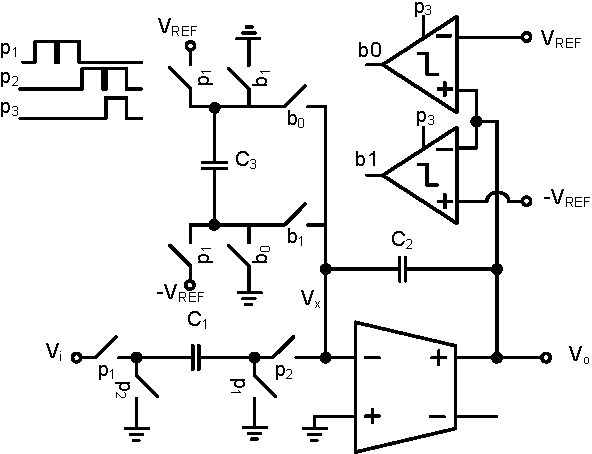
\includegraphics[width=\myfigwidth]{graphics/sc_mod}}
  \caption{Switched-capacitor modulo integrator}
  \label{sdrfig:scmod}
\end{figure}

If $C_1 = C_2 = C_3$ the charge transfer equations implement the
modulo defined in \req{modintdef}. The modulo operation ensures that the
output signal in $p_3$ stays within $V_{o} \in \langle -V_R/2, V_R/2
\rangle$ as long as $V_{i} \in \langle -V_R/2, V_R/2 \rangle$. 

%-------------------------------------------------------
\subsection{Effects of finite gain in modulo integrators}
%-------------------------------------------------------
One of the non-idealities in SC integrators is the
finite opamp gain. The effects of finite opamp gain was covered in \cite{temes80} and
\cite{martin81}.  The transfer function of an integrator with finite
gain can be approximated by 

\eqn{
\label{sdreq:zgainmodap}
\frac{V_o(z)}{V_i(z)} = \dfrac{C_1}{C_2}\dfrac{ a z^{-1}}{1 - b z^{-1}}
}
where
\eqna{
  a &{} = {}& 1-\dfrac{1+C_1/C_2}{A_0}\\
  b &{} = {}& 1-\dfrac{1}{A_0} 
}
and $A_0$ is the DC gain of the opamp. The derivation of this is included in \myappname
\ref{sdrap:intgain}. A block 
model of the modulo integrator is shown in Fig. \ref{sdrfig:modint_beh}.

\begin{figure}[htbp]
\centerline{ 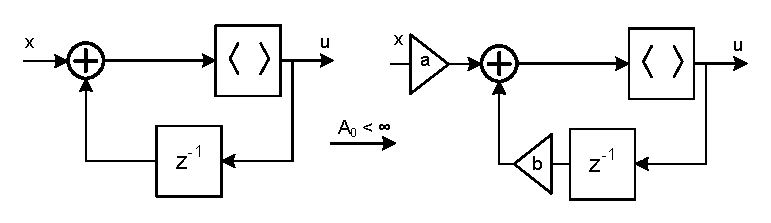
\includegraphics[width=\myfigwidth]{graphics/modint_beh}}
  \caption{ Block model of the modulo integrator for finite DC gain.}
  \label{sdrfig:modint_beh}
\end{figure}

We have assumed that the modulo operation does not influence the
effects of finite gain. To verify the model in
Fig. \ref{sdrfig:modint_beh}  it is implemented in \simulink \cite{simulink} and compared
with two other models, one based on the difference equations
and one based on a SPICE implementation.

An expression can be
derived for the output of a first-order OLSDM using the modulo
arithmetic used in Section \ref{sdrbasicmodulo}. The output of a first
order OLSDM with finite DC gain in the modulo integrators can be
approximated by the difference equation
\eqn{
\label{sdreq:modoutgain}
  y_n = \left \langle x_{n-1} - \dfrac{q_{u,n}}{A_0} + q_n - q_{n-1} \right \rangle_R
}
where $q_{u,n}$ is a white noise approximation of the modulo
integrator output $u_{n}$. The derivation is left for \myappname
\ref{sdrap:finitegain}. 

The
difference between \req{modoutgain} and \req{modout3} is the term $-q_{u,n}/A$. Due to the finite
opamp gain  there is a leakage of $u_n$ to the
output. The modulo integrator output ($u_n$) is a deterministic signal of the input, but we assume it
can be approximated as quantization noise with the limits $q_{u,n} \in
\langle -R/2, R/2 \rangle$. 


From \req{modoutgain} the \textit{signal-to-noise 
and distortion ratio} (SNDR) can be
calculated. For a sinusoidal input the SNDR is
\eqn{
\label{sdreq:osdsndr}
SNDR =  10 \log \left(\frac{A^2/2}{\dfrac{1}{12A_0^2 OSR} +
    \dfrac{LSB^2}{12}\times K}\right)
}
where $A$ is the amplitude of the sinusoid, the first term in the
denominator is the effects of finite gain, and the second term the
quantization noise where $K = 2
\int_0^{f_s/2OSR}{|NTF(z=e^{j\omega})|^2}df$. The calculation of
\req{osdsndr} is left for \myappname \ref{sdrap:sndr}. With $B=7$, $OSR=4$
and $A_0=50dB$ the expected SNDR is 51.3dB. 

%  The two models
% \req{zgainmod} and \req{modoutgain} were compared in a behavioral
% level \matlab simulation. Equation \req{zgainmod} was implemented as
% a z-domain SIMULINK model and Equation \req{modoutgain} was
% implemented as a discrete time difference equation in \matlab. Fig.
% \ref{sdrfig:gainmodel} shows the comparison of the two models and the
% calculated value. Each data point represent the SNDR extracted from a
% $2^{15}$ point FFT for a given input signal frequency. The approximation in \req{modoutgain} differs from
% the calculated value, \req{osdsndr}, because the random values set $q_u$
% in \req{modoutgain}  are chosen randomly from frequency point to frequency
% point. But as we can see from Fig. \ref{sdrfig:gainmodel} the
% approximation has the calculated value as the mean. The z-domain
% model is a more accurate model since it is the signal $u_n$ that leaks
% to the output and not  white noise approximation. As expected the SNDR
% is sligthly higher in the SIMULINK model, since the power of the
% signal $u_n$ is less than the power of $q_{u,n}$. There is also a
% frequency dependence in the SNDR in the SIMULINK model. For low
% frequency input the approximation $u_n \approx q_{u,n}$ is better and
% we see the SNDR aproach eachother. Accordingly, \req{zgainmod} is a
% valid model for the modulo integrator.

%The difference between the SNDR of the two models is
%  less than 1\% for an $OSR=4$, a 7-bit quantizer and a DC gain of
%  40dB. This fortifies the assumption that previous derivations of
%  effects of DC gain can be applied to modulo integrators. 

% \begin{figure}[htbp]
% \centerline{ 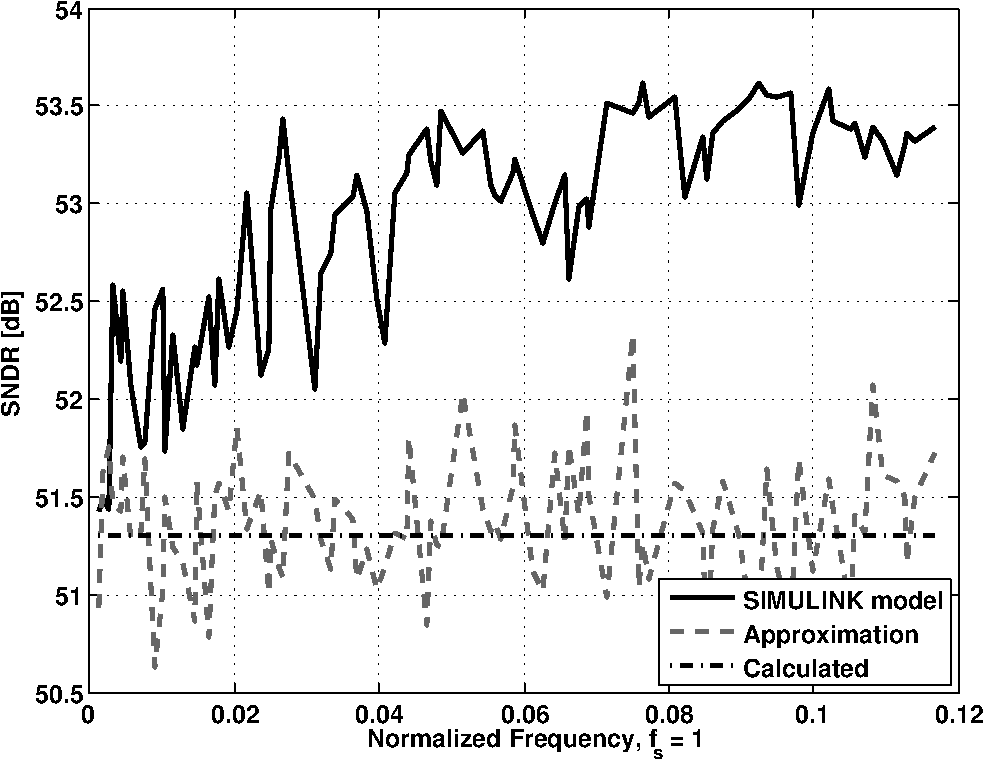
\includegraphics[width=\myfigwidth]{gainmodel}}
%   \caption{ z-domain model of the modulo integrator with DC gain $A < \infty$.}
%   \label{sdrfig:gainmodel}
% \end{figure}

%Fig. \ref{sdrfig:intmod} shows a comparison between the models of the
%low-pass first-order OLSDM (shown in Fig. \ref{sdrfig:olsdm-basic}).
An FFT of the \simulink model (Fig. \ref{sdrfig:modint_beh}) is shown in
Fig. \ref{sdrfig:intmod_z}. Fig. \ref{sdrfig:intmod_d} shows the FFT of the
approximate model as defined by \req{modoutgain}. The FFT of the SPICE model output is shown in
Fig. \ref{sdrfig:intmod_spice}.

 The
approximation in Fig. \ref{sdrfig:intmod_d} is different from the others, here
the noise floor is relatively flat up to $0.01f_s$. At that
point the shaped quantization noise is larger than the leakage from the
integrator output (from \req{modoutgain}) and we get
the high-pass noise shaping. 

For both the \simulink model in Fig.
\ref{sdrfig:intmod_z} and SPICE model in Fig. \ref{sdrfig:intmod_spice} we can
see that the contribution $q_{u,n}/A_0$ is not white, but 
equal to $u_n/A_0$.  Fig. \ref{sdrfig:intmod_u} shows the FFT
of the modulo integrator output ($u_n$) from the \simulink simulations.

The vertical line in the figures denote the
upper bandwidth limit for noise calculation. As a quick estimate of the performance
\req{osdsndr} works well. It overestimates the effects of noise and
has an SNDR of 51.3dB compared to 52.2dB for the \simulink model,
51.66dB in the SPICE model and 51.44dB for the approximation
\req{modoutgain}.  These models show that the modulo operation does
not significantly influence the equations for the effects of finite gain.

Calculation speed is very different in the three models. Calculating \req{osdsndr} takes less than
a second, while the \simulink model take ten seconds for $2^{15}$
points, and the SPICE
simulations take a thousand seconds for $2^{15}$ points. 

To increase the resolution of this first order low-pass OLSDM we can either increase
the quantizer resolution, which we will not do, or reduce the in-band quantization
noise with higher order noise shaping. To get higher order
noise shaping we can increase the
number of zeros in the noise transfer function (NTF) of the
modulator. Either at z=1 (zero frequency) with modulo integrators, or  introduce
zeros at non-zero frequencies. The next section introduces the modulo
resonator, which is used to insert a zero at a non-zero frequency in
the noise transfer function.

\mymodintfig

 
-----------------------------------------------------



%########################################################################
\section{Modulo resonator}\label{sdrmoduloresonator}
%########################################################################

Zeros at non-zero frequency in the noise transfer function reduce the oversampling
ratio for a given quantizer resolution. With zeros at non-zero frequency one can 
implement band-pass sigma-delta modulators. In this section the modulo
resonator is introduced and the ideal and simulated performance
is discussed. 

A model of modulator with zeros at non-zero
frequency can be seen in Fig. \ref{sdrfig:sdrideal}. 
In a world
without signal swing limitations the input signal ($x_n$) can be conditioned
with a resonator, the output of the resonator quantized, and input
signal restored
with a notch filter. The quantization noise will pass through
the notch filter and be filtered accordingly. The output of the
modulator is written as
\eqn{
  Y(z) = STF(z)X(z) + NTF(z)Q(z) 
}
 $STF(z)$ is the signal
transfer function and $NTF(z)$ is the
noise transfer function. 

The input signal pass through
unchanged if the notch filter response matches
the resonator response, thus $STF(z) = 1$.\footnote{The $STF(z)$ will
  probably also contain a time delay, depending on the
  implementation, $STF(z) = z^{-n}$}

 In Fig.
\ref{sdrfig:sdrideal} the $NTF(z)$ is equal to the notch filter response,
which has
a zero at a non-zero frequency.

\begin{figure}[htbp]
\centerline{ 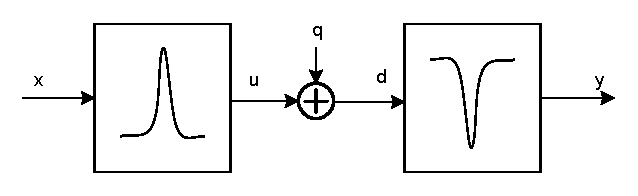
\includegraphics[width=\myfigwidtha]{graphics/sdr_ideal}}
  \caption{Ideal open-loop implementation of NTF zeros at non-zero frequency}
  \label{sdrfig:sdrideal}
\end{figure}

A common resonator used in sigma-delta modulators is based on the lossless discrete
integrator (LDI) \cite{bruton75} shown in Fig. \ref{sdrfig:sdldi}. The
LDI resonator has
a pair of complex conjugate poles at 
\eqn{
  z_p  = \rho \pm j\sqrt(1-\rho^2), \rho = 1-g/2
}
and a resonance frequency of $\omega_0 = cos^{-1}(\rho)$. The
advantage of the LDI is the tunable resonance
frequency. 

\begin{figure}[htbp]
\centerline{ 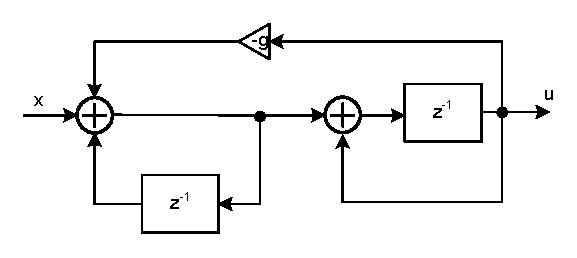
\includegraphics[width=\myfigwidthb]{graphics/sd_ldi}}
  \caption{Resonator based on the lossless discrete integrator (LDI)}
  \label{sdrfig:sdldi}
\end{figure}

If the 
integrators in Fig. \ref{sdrfig:sdldi} are replaced with modulo integrators
we get the modulo resonator shown in
Fig. \ref{sdrfig:sdr_ldi}.  With this modulo resonator 
we can implement Fig. \ref{sdrfig:sdrideal} as shown in
Fig. \ref{sdrfig:sdr_mod}. Fig. \ref{sdrfig:sdr_mod} is a modulo resonator followed by a
linear quantizer and a modulo
notch filter. The modulo operations at the end of the notch filter
reverse the modulo in the resonator. We use two modulo functions in
the notch filter since the modulo is defined as  \req{modintdef}.

%Note that from \req{prop1} we
%should only require one modulo, but the modulus used in Fig. \ref{sdrfig:sdr_mod} are
%defined as \req{limmodulo}.
% The modulo in Fig. \ref{sdrfig:sdr_mod} subtracts or adds
%the range R  once if  $|x_n| \geq R/2$, not infinitely many times as
%\req{modulo}. 

\begin{figure}[htbp]
\centerline{ 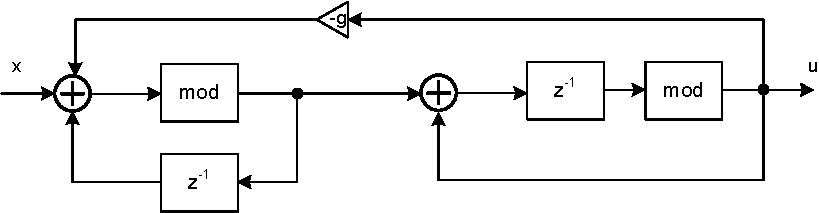
\includegraphics[width=\myfigwidth]{graphics/sdr_ldi}}
  \caption{The modulo resonator }
  \label{sdrfig:sdr_ldi}
\end{figure}

\begin{figure}[htbp]
\centerline{ 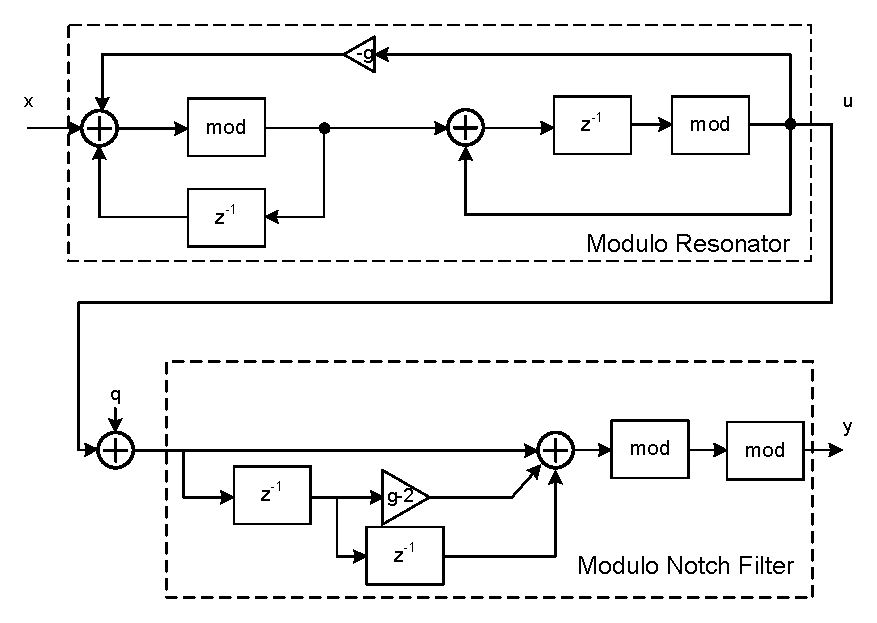
\includegraphics[width=\myfigwidth]{graphics/sdr_mod}}
  \caption{The open-loop sigma-delta modulator with NTF zeros at
    non-zero frequency}
  \label{sdrfig:sdr_mod}
\end{figure}


\begin{figure}[htbp]
\centerline{ 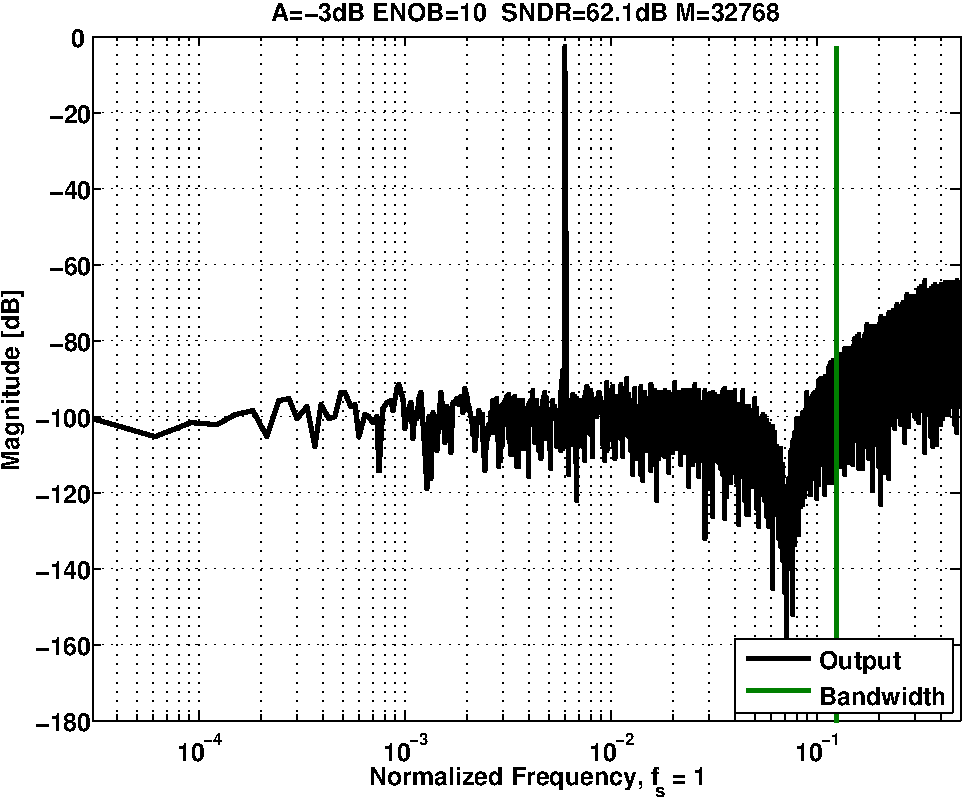
\includegraphics[width=\myfigwidth]{graphics/osdr}}
  \caption{Modulator response. Magnitude of a $2^{15}$ point
    FFT. Input signal amplitude is -3dBFS, input signal frequency is
    at $f_i = 0.006$ with a normalized sampling frequency, $f_s=1$.
  The SNDR with $OSR=4$ is 62.1dB}
  \label{sdrfig:osdr}
\end{figure}


The noise transfer function of the modulator in Fig.
\ref{sdrfig:sdr_mod} is
\eqn{
  NTF(z) = z^2 + (g-2) z + 1
} 
And has an ideal SNDR of 
\eqn{
\label{sdreq:sndr}
SNDR =  10 \log \left(\frac{A^2/2}{2\int_0^{f_s/2OSR}{Q_M^2(f) |NTF(z)|^2}df}\right)
}
if we assume sinusoidal input. Here $Q_M^2(f)$ is the power spectral density of the quantization noise
given by
\eqn{
  Q_M^2(f) = \frac{LSB^2}{12f_s} = \frac{1}{2^{2B}12 f_s}
}
where $LSB = R/2^B$ and $R=1$. 


The optimum zero frequency can be calculated from \req{sndr}. Using an
OSR of four the optimum zero frequency is
$f_i = 0.0718 f_s$ ($g=0.2$). Calculation of the optimum zero
frequencies was covered in detail in \cite{schreier93}.


Fig.
\ref{sdrfig:sdr_mod} was implemented as a \simulink model.
 Fig. \ref{sdrfig:osdr} is a $2^{15}$ point
FFT of the modulator output ($y_n$) with an input signal amplitude of -3dBFS and a
quantization noise power equivalent
to a 7-bit quantizer. Coherent sampling and a Hanning window was used
to avoid spectral leakage of the signal power into neighboring FFT
bins. A brick-wall filter with bandwidth from $0 - f_s/2OSR$ was
used to calculate the SNDR. The
vertical line in Fig. \ref{sdrfig:osdr} denotes the bandwidth. 


For $f_s=1$,
$OSR=4$, $B=7$, $A=1/\sqrt{8}$ the ideal SNDR from \req{sndr} is
62dB. The simulated SNDR match the 
ideal SNDR (1\% difference). 

\subsection{Effects of finite gain in modulo resonators}
Exact analysis of the effects of finite gain in a modulator with a modulo resonator
is complex. The derivation is left for \myappname \ref{sdrap:modresgain}. 

The modulator output
($y_n$ in Fig. \ref{sdrfig:sdr_mod})
 with finite gain in the modulo resonators can be approximated by
\eqn{
  \label{sdreq:modresoest}
  y_n \approx \langle x_{n-1} + (1+g)\epsilon_{p,n-1} + e_n\rangle_R
}
where $\epsilon_p$ is the leakage from the first modulo integrator. The shaped quantization noise is
represented by $e_n$. 
The leakage from the first modulo integrator dominate over the leakage from
the second modulo integrator if the opamp gains in the two
integrators are equal. 


With \req{modresoest} the SNDR is 
\eqn{
\label{sdreq:resapprox}
  SNDR \approx 10 \log\left(\dfrac{ A^2/2}{\dfrac{(1+g)^2}{12
        A_0^2}\dfrac{1}{OSR} + \dfrac{LSB^2}{12}\times K}\right)
}
where $K = \int_0^{f_s/2OSR}|NTF(z)|^2df$. 

Accuracy of
\req{resapprox} depend on the DC gain. It overestimates the SNDR with
1.5dB to 1dB for a DC gain of 60dB - 80dB compared to the
derivation in \myappname \ref{sdrap:modresgain}. But the leakage from the  modulo integrator
is approximated by a white noise source, which  has higher
power than the  power of the actual leakage. Accordingly, the two assumptions: leakage
approximated by a
white noise source, and assuming $\epsilon_p$ is the dominating noise
source, work in opposite directions.

 For
A=-3dBFS, $OSR=4$, $g=0.2$, $LSB=1/2^7$ and a DC gain of
60dB, the approximate SNDR from 
\req{resapprox} is 59.5dB. Whereas for 40dB DC gain the SNDR is
43.1dB. 

Using the previously described modulo integrators in a \simulink
model of
the modulator from Fig. \ref{sdrfig:sdr_mod}, the SNDR is 59.2dB for
60dB DC gain and
42.5dB  for 40dB DC gain. A difference of 0.3dB (4\%) at 60dB DC
gain and 0.6dB (7\%) at 40dB DC gain.

%The next section show how a modulo resonators are combined with
%modulo integrator to produce a more realistic OLSDM, a fifth-order
%low-pass OLSDM with an 
%OSR of four and an ideal SNDR of 85dB.

%########################################################################
\section{Fifth-order low-pass OLSDM}\label{sdrmatlabsim}
%########################################################################
It has previously been shown that the
accuracy of SC circuits depend on the capacitor mismatch, finite DC
gain and unity-gain bandwidth of the opamp
\cite{temes80},\cite{martin81}. We have discussed the effects of
finite DC gain, but left the derivation of capacitor mismatch and
finite unity-gain bandwidth for later
work. But we expect the effects to be similar and limit
the performance to below 14-bit ENOB. This assumes no calibration or
trimming. 

Stages in an OLSDM can be pipelined and it is possible 
to use high latency quantizers such as pipelined ADCs or SAR ADCs. One
in envisioned application of OLSDM is a 14-bit high speed ( 20MS/s) ADC. 
In this section we describe a fifth-order OLSDM with an OSR
of four and 13-bit ENOB.

%-------------------------------------------------------
\subsection{Ideal modulator}
%-------------------------------------------------------
The modulator is  seen in Fig.
\ref{sdrfig:osdr3}. It has two modulo resonators, a
modulo integrator, a 7-bit quantizer, a modulo differentiator, and
two modulo notch filters. To ensure that \req{inlimit} is satisfied 
a gain of 0.9 is inserted between the first and second resonators,
and between the second resonator and the modulo integrator (this is not shown in Fig.
\ref{sdrfig:osdr3}). 

\begin{figure}[htbp]
\centerline{ 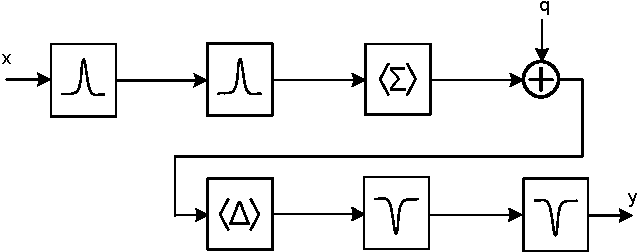
\includegraphics[width=\myfigwidth]{graphics/osdr21_sch}}
  \caption{Fifth-order open-loop sigma-delta modulator}
  \label{sdrfig:osdr3}
\end{figure}

The noise transfer function of the modulator in Fig. \ref{sdrfig:osdr3} is given by
\eqn{
\label{sdreq:fifth_ntf}
  NTF(z) = \frac{(z^2 +(g_1-2)z+1)(z^2 +(g_2-2)z+1)(z-1)}{0.81}
}
And the ideal SNDR can be calculated with \req{sndr}, using the
NTF from \req{fifth_ntf}. With an OSR of four the optimal constants  
are $g_1 = 0.17$ and $g_2 = 0.48$. For $OSR=4$, A=-3dBFS and $B=7$
the ideal SNDR is 85dB. 

A $2^{15}$ point FFT is calculated
from the output of a \matlab simulation of the ideal modulator in Fig. \ref{sdrfig:osdr3}. The FFT
is shown in Fig. \ref{sdrfig:osdr3_ideal}. The simulated match the ideal
SNDR (1\% difference).

The input signal
must be limited as stated in \req{inlimit}.
An input signal amplitude of
-3dBFS $= 1/\sqrt{8} \approx 0.354$ is used in the
simulations.  If we insert for $N=5$
and $B=7$ in the input signal limit \req{inlimit}
\eqn{
  |x(n)| < R(1/2 - 2^{5-1}/2^7) = 0.375
}
Thus the modulator is valid for an input signal amplitude of
-3dBFS.

%The ideal SNDR of the modulator in Fig. 
%\ref{sdrfig:osdr3} is 80.98dB for 
%$A=1/\sqrt{8}$, $OSR=4$, $B=7$ and $f_s=1$. 
%The simulated SNDR =
%80.98dB, which matches the ideal SNDR. 

\begin{figure}[htbp]
\centerline{ 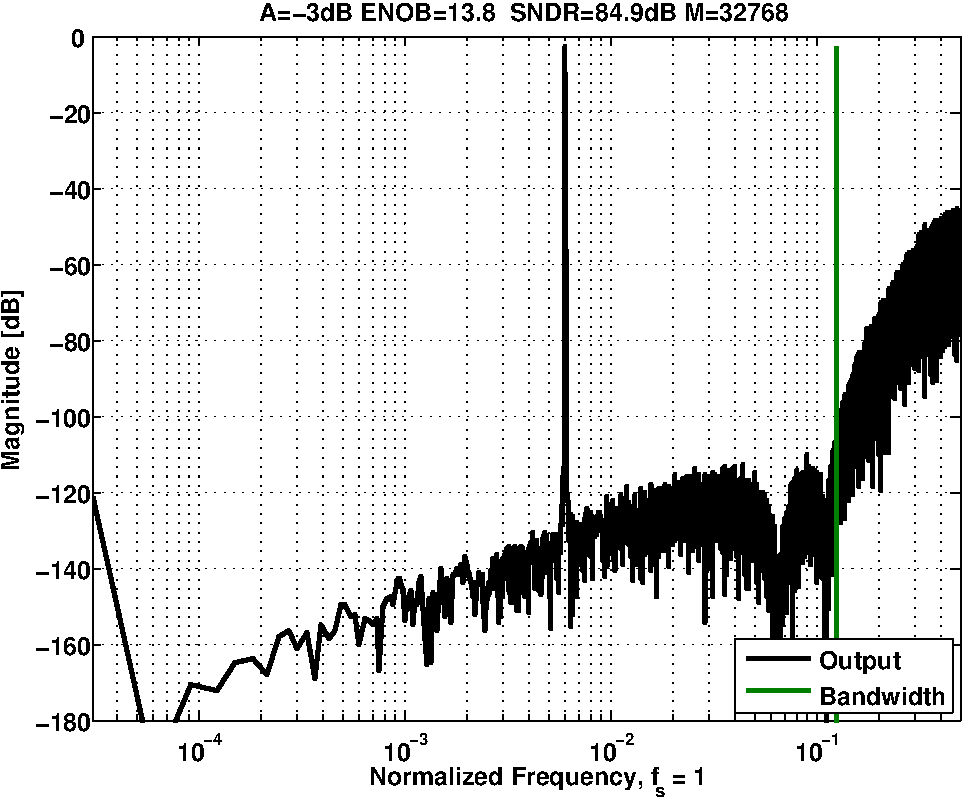
\includegraphics[width=\myfigwidth]{graphics/osdr21}}
  \caption{Modulator output. Magnitude of a $2^{15}$ point FFT of the
    modulator output. Input signal amplitude -3dBFS. Input frequency
    $f_i = 0.006$ and sampling frequency $f_s = 1$. With an $OSR=4$
    the SNDR is 84.9dB }
  \label{sdrfig:osdr3_ideal}
\end{figure}

%-------------------------------------------------------
\subsection{Modulator with finite opamp gain in modulo integrators}
%-------------------------------------------------------
Fig. \ref{sdrfig:osdr3g} shows the fifth order sigma-delta modulator with the
the modeled opamp gain. The modulo integrators are
modeled with an
opamp gain
of 85dB in the first resonator, 75dB in second resonator, and 65dB
in the last modulo
integrator. These gains were chosen from design equations based on \req{resapprox}.
Assume the leakage due to 
finite opamp gain in the first modulo resonator dominate. The SNDR is
then estimated from \req{resapprox}. The estimated SNDR for
this modulator is 83.3dB for an input amplitude of -3dBFS.
Fig.
\ref{sdrfig:osdr374} is a $2^{15}$ point FFT of the modulator output ($y_n$)
using an input signal amplitude of -3dBFS. 

\begin{figure}[htbp]
\centerline{ 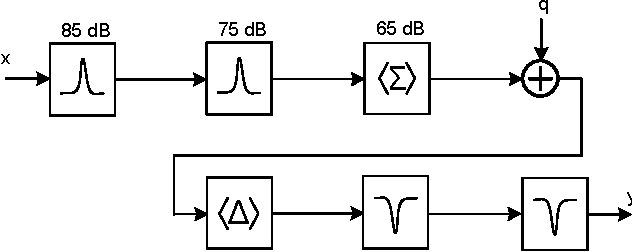
\includegraphics[width=\myfigwidth]{graphics/osdr21g_sch}}
  \caption{Fifth-order open-loop sigma-delta modulator. The DC gain of
    opamps are shown above the stages.}
  \label{sdrfig:osdr3g}
\end{figure}


\begin{figure}[htbp]
\centerline{ 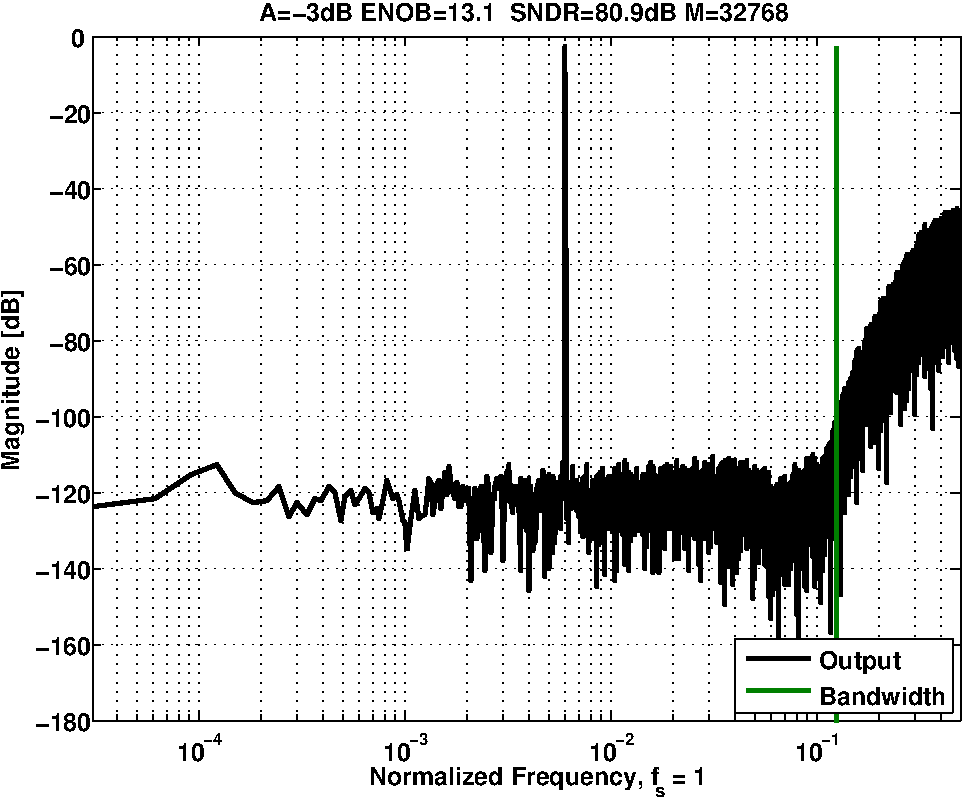
\includegraphics[width=\myfigwidth]{graphics/osdr21g}}
  \caption{Magnitude of a $2^{15}$ point FFT of the modulator
    output. Input signal amplitude -3dBFS, input frequency $f_i =
    0.006$ and sampling frequency $f_s = 1$. With an $OSR=4$ the SNDR=80.9dB}
  \label{sdrfig:osdr374}
\end{figure}

The simulated SNDR is
 80.9dB (13.15-bit ENOB\footnote{ENOB = (SNDR-1.76)/6.02}), or 2.4dB below the estimated SNDR. This is expected due to
leakage from later stages. If we increase the DC gain in the second
modulo resonator and the last modulo
integrator to 200dB, we remove
them as noise contributors. This increases the SNDR to 82.8dB, which
is 0.5dB (6\%) lower than the estimated. 

The
modulator in Fig. \ref{sdrfig:osdr3g} was implemented in SPICE as a switched
capacitor circuit. 



%-------------------------------------------------------
\subsection{Switched capacitor modulator}
%-------------------------------------------------------
Fig.
\ref{sdrfig:osdr3spice} shows a switched-capacitor implementation of
the modulator. A single ended modulator was used for simplicity. 
\begin{figure}[htbp]
\centerline{ 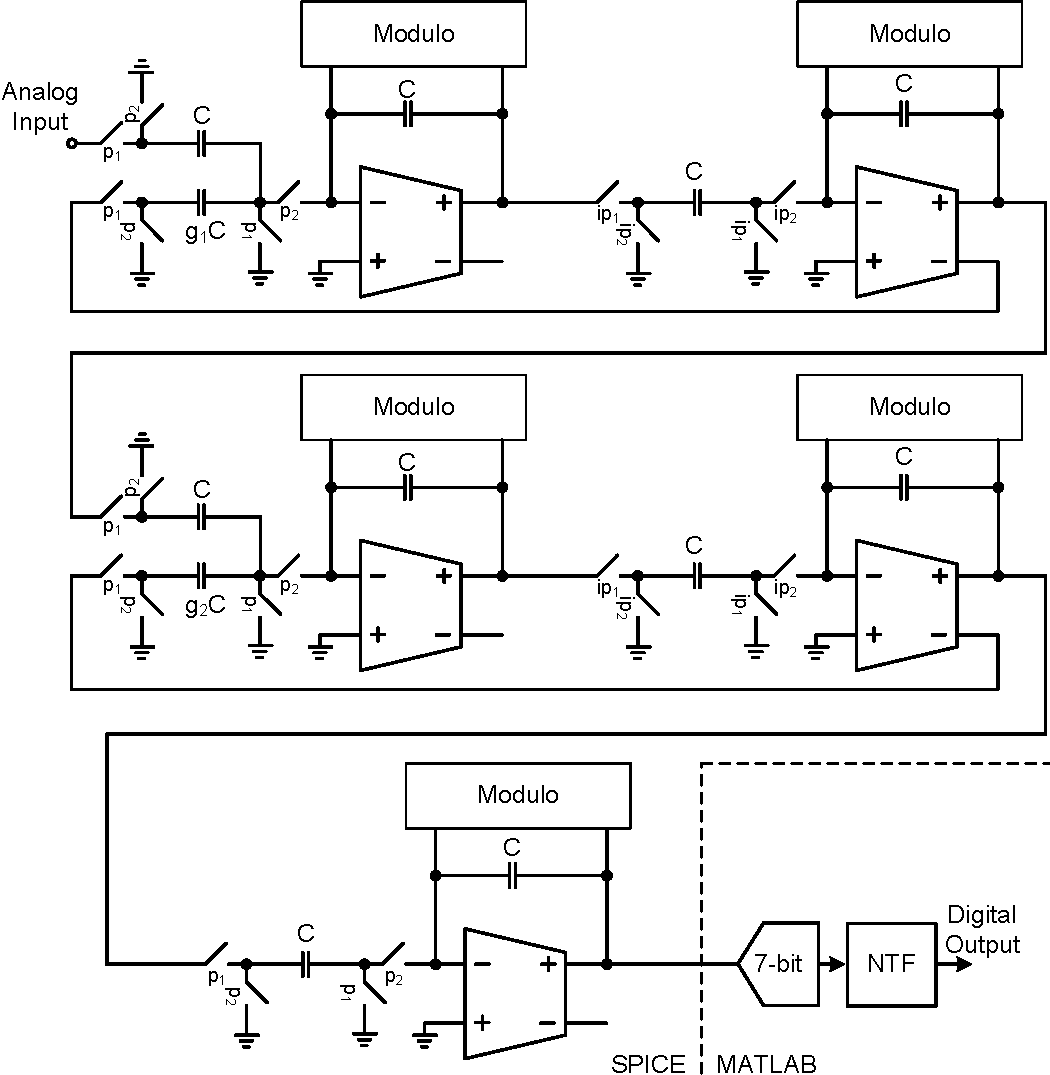
\includegraphics[width=\myfigwidth]{graphics/osdr21_spice_sch}}
  \caption{Fifth order OLSDM SPICE model. Quantization and NTF are implemented in \matlab}
  \label{sdrfig:osdr3spice}
\end{figure}

The opamps have a DC gain of 85dB, 85dB, 75dB, 75dB, and 65dB.
The opamp was implemented as a macro-model of a single-pole operational amplifier.

A
comparison between the \matlab model and the SPICE model is shown in
Fig. \ref{sdrfig:fifthordersdm}, here a $2^{15}$ point FFT was run on both
the SPICE and the \matlab outputs. The SNDR is the same for both
models. In SPICE, however, there is more harmonic content, with the second
harmonic visible in the FFT.

The quantizer and NTF for the SPICE simulations is implemented in
\matlab. A 7-bit ideal quantizer is used instead of the linear
approximation to quantization noise. 

\begin{figure}[htbp]
\centerline{ 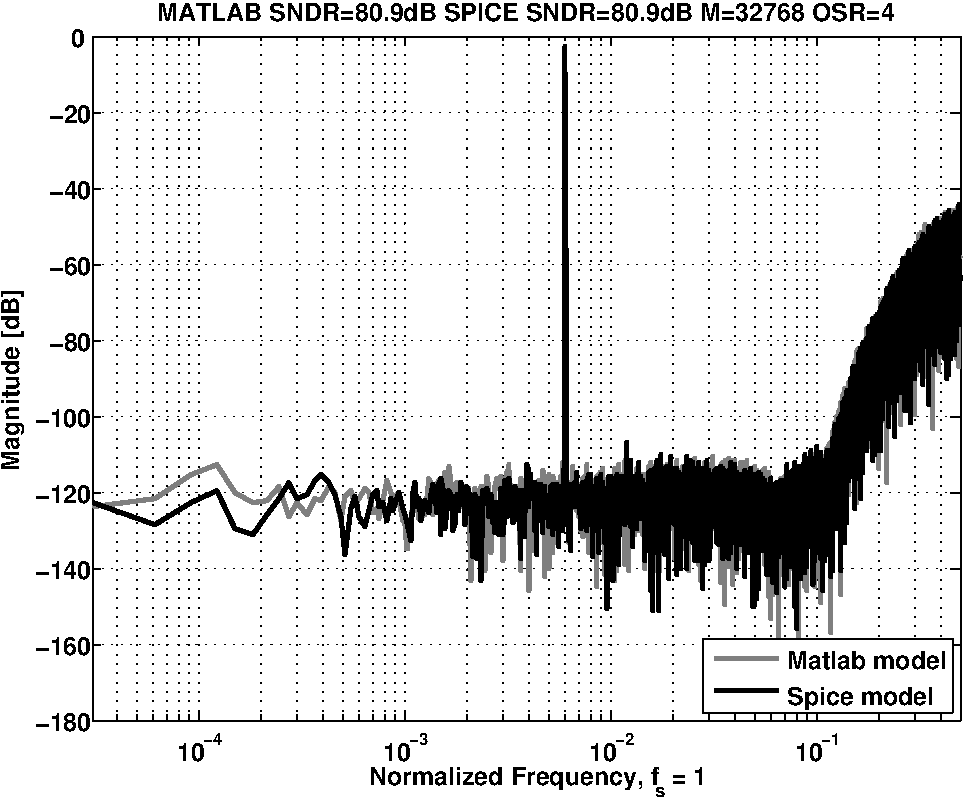
\includegraphics[width=\myfigwidth]{graphics/osdr21_spice}}
  \caption{Comparison of SPICE model and \matlab model. Input signal amplitude -3dBFS, input frequency $f_i =
    0.006$ and sampling frequency $f_s = 1$. With an $OSR=4$ the
    SNDR is 80.9dB for the \matlab model and 80.9dB for the
    SPICE model.}
  \label{sdrfig:fifthordersdm}
\end{figure}

\subsubsection{Capacitor mismatch}
In modern CMOS processes the matching between capacitors is good. In a
typical 90nm process the matching of two 10pF Metal-Insulator-Metal
(MIM) capacitors can be as good as 0.06\% (3 sigma). In the
switched-capacitor OLSDM matching will influence the coefficients, and
the inter-stage gain. The matching in the first stage is most critical,
as mismatch in later stages is attenuated by the gain of the previous
stage. With a mismatch in the coefficients and inter-stage gain the
digital transfer function (from the quantizer and out) will not have
the correct coefficients. This will lead to noise
leakage, since the poles of the analog filter (the two resonators and
the integrator) will not match the zeros in the digital filter (the
two notch filters and the differentiator). 

With 0.06\% matching between capacitors the SNDR degrades to 79.7dB, which is not
significant. But the capacitor sizes in a switched-capacitor
implementation will be determined by the most critical capacitor, the
$g_1C$ capacitor in the first stage. In this example $g_1 = 0.17$,
which is small. With mismatch taken into consideration it might be
advantageous to move resonator with the $g_2 = 0.48$ first, even
though this will increases the noise leakage somewhat. The unit capacitor
$C$ can be chosen smaller since the $g_2C$ capacitor must match to
0.06\% (3 sigma). With $g_1C$ as the first capacitor the unit capacitor must be
almost three times larger than if the $g_2C$ capacitor is used as the
first capacitor.

\subsubsection{Comparator Offset}
 A concern with a switched-capacitor implementation is the offset in
 the comparators used in the modulo resonator. Simulations suggest
 that the stochastic offset of comparators in the modulo resonator
 must be within 0.25\% of full-scale to have an SNDR of
 above 77dB. Achieving an offset on this level requires rigorous analog
 design. At offset of 1\% of full-scale the SNDR degrades
 to 65dB. For example, with a full-scale of 2V peak-to-peak we tolerate
 an offset of $\pm 5mV$ in the comparator thresholds.


%74dB osdr3_l -6dB 11.05 vs 11.04 in model with N=2048



%########################################################################
\section{Conclusion}
%########################################################################
In this paper we introduced the modulo resonator for open-loop
sigma-delta modulators (OLSDM). It was used with a modulo notch filter to
introduce a zero in the noise transfer function at a non-zero
frequency. The modulo resonator and previously published modulo
integrator were used in a behavioral model of a switched-capacitor fifth-order OLSDM with more
than 13-bit effective number of bits for an oversampling ratio of
four. We proved that the number of bits in the quantizer (B) must be
larger than the order of the modulator (N) to ensure equivalence between OLSDM and sigma-delta
modulation.


%\appendices
\myappendices

\section{Proof  of  modulo theorem}
\label{sdrap:modproof}
\begin{IEEEproof}
From definition 
\eqn{
\label{sdreq:roundmodulo}
\langle a + nR\rangle_R = \langle a \rangle_R
}
where $n$ is an integer. Given
\eqn{
  \langle \langle x \rangle_R + \langle y \rangle_R \rangle_R
}
we can write $\langle x \rangle_R = x-nR$ and $\langle y \rangle_R = y
- mR$, where $n$ and $m$ are integers. From \req{roundmodulo} it follows that
\eqn{
  \langle x - nR + y - mR \rangle_R = \langle x + y \rangle_R
}
\end{IEEEproof}

\section{Effects of finite gain in SC integrators}
\label{sdrap:intgain}
If we assume infinite DC gain in the opamp the
charge transfer equation is simply
\eqn{
\label{sdreq:intchargez}
  C_2 V_{o,n} = C_2 V_{o,n-1}  + C_1 V_{i,n-1}
}
The z-domain transfer function of  \req{intchargez} is
\eqn{
\label{sdreq:intzdomain}
\frac{V_o(z)}{V_i(z)} = \frac{C_1}{C_2}\frac{z^{-1}}{1-z^{-1}}
}
If $C_1 =C_2$, then \req{intzdomain} is the well known transfer function of
a discrete time integrator and is a good approximation if the
DC gain ($A_0$) is much higher than the accuracy required. If the DC gain is close to,
or lower than the accuracy, then \req{intzdomain} no longer applies.

With finite opamp gain the voltage $V_x$ (in Fig. \ref{sdrfig:scint}) will be different from
zero. A non-zero $V_x$
will result in  a
residual charge on capacitor $C_1$ given by $Q_{1,n} = C_1
V_x$. The
charge transfer equation change into
\eqn{
\label{sdreq:chgain}
  Q_{2,n} = Q_{2,n-1} + Q_{1,n-1} + Q_{1,n}
}
where $Q_2 = C_2 (V_o - V_x)$, $Q_{1,n-1} = C_1 V_i$. The residual
voltage $V_x$ is equal to $V_x = -V_o/A_0$. We define
\eqn{
\alpha = 1 + \frac{1}{A_0}
}
If we expand \req{chgain} we get
\eqn{
\alpha V_{o,n}  = \alpha V_{o,n-1}  + \frac{C_1}{C_2}
V_{i,n-1} - \frac{C_1}{C_2} \frac{V_{o,n}}{A_0}
}
Solved for $V_o/V_i$ and transferred to the z-domain we get the
transfer function
\eqn{
\label{sdreq:zgainexact}
\frac{V_o(z)}{V_i(z)}  = \dfrac{C_1}{C_2} \dfrac{\left(\dfrac{1}{1 + \dfrac{1+
      C_1/C_2}{A_0}}\right)z^{-1}}{1 - \alpha \left(\dfrac{1}{1 + \dfrac{1+
      C_1/C_2}{A_0}}\right) z^{-1}}
}
If we assume $A_0>>1$, then \req{zgainexact} can be approximated to first
order by
\eqn{
\label{sdreq:zgainmodap1}
\frac{V_o(z)}{V_i(z)} = \dfrac{C_1}{C_2}\dfrac{\left(1 -
  \dfrac{1+C_1/C_2}{A_0}\right)z^{-1}}{1 - \left(1 - \dfrac{1}{A_0}\right) z^{-1}}
}

\section{Effects of finite gain in modulo integrators}
\label{sdrap:finitegain}
From charge transfer equations the output of the modulo integrator is
\eqn{
  \alpha u_n = \left \langle \alpha u_{n-1} + x_{n-1} - u_n/A_0 \right \rangle_R
}
where $\alpha  = 1+1/A_0$ and $A_0$ is the DC gain of the opamp. We
also have
\eqn{
  \alpha u_{n-1} = \left \langle \alpha u_{n-2} + x_{n-2} - u_{n-1}/A_0 \right \rangle_R
}
and that
\eqn{
  \alpha u_{n-2} = \left \langle \alpha u_{n-3} + x_{n-3} - u_{n-2}/A_0 \right \rangle_R
}
Using \req{prop1} the output of the modulo integrator is 
\setlength{\arraycolsep}{0.0em}
\begin{eqnarray}
\label{sdreq:apintout}
u_n &{}={}& \dfrac{\left \langle \sum_{i=0}^\infty{x_{n-1-i}\alpha^i} -
  \sum_{i=0}^\infty{\dfrac{u_{n-i}}{A_0}\alpha^i} \right \rangle_R}{\alpha}\nonumber\\
&{}={}& \left \langle \sum_{i=0}^\infty{x_{n-1-i}\alpha^{i-1}} -
  \sum_{i=0}^\infty{\dfrac{u_{n-i}}{A_0}\alpha^{i-1}} \right \rangle_R\nonumber\\
\end{eqnarray}
\setlength{\arraycolsep}{5pt}

The output of the modulator is 
\eqn{
y_n = u_n - u_{n-1} + q_n - q_{n-1}
}
using \req{prop1} and \req{apintout}
\eqn{
 y_n = \left \langle \dfrac{x_{n-1}}{\alpha} - \dfrac{u_n}{A_0\alpha} +
 q_n - q_{n-1} \right \rangle_R
}
Assuming $A_0 >> 1$ we can approximate the modulator output by
\eqn{
\label{sdreq:modapprox1}
  y_n = \left \langle x_{n-1} - \dfrac{u_n}{A_0} + q_n - q_{n-1} \right \rangle_R
}
The signal $u_n$  can be
written as \req{modint_copy}. This signal is the quantization noise
after rounding the integrator output to the range R. We assume this
quantization noise is white. Assume $u_n \approx q_{u,n} \in \langle -R/2,
R/2 \rangle$. Then \req{modapprox1} simplifies to 
\eqn{
\label{sdreq:modapprox2}
  y_n = \left \langle x_{n-1} - \dfrac{q_{u,n}}{A_0} + q_n - q_{n-1} \right \rangle_R
}

\section{Calculation of the SNDR}
\label{sdrap:sndr}

The power spectral density of quantization noise is given by the
well known equation
\eqn{
  Q^2(f) = \dfrac{LSB^2}{12 f_s}
}
where $f_s$ is the sampling frequency. For a given bandwidth the noise
power is
\eqn{
  Q^2 = 2\int_0^{f_s/2OSR} Q^2(f)df = \dfrac{ LSB^2}{12}\dfrac{1}{OSR}
}
The LSB of $q_{u,n}/A_0$ can be written as $R/A_0$. And if we assume $R=1$
the noise power of the modulo integrator output leakage is given by
\eqn{
\label{sdreq:osdnu}
  Q_u^2 = \dfrac{1}{12 \times A_0^2}\dfrac{1}{ OSR}
}   
The quantization noise in a first order OLSDM is high-pass filtered, and has a
noise transfer function of
\eqn{
  NTF(z) = 1-z^{-1}
}
The LSB of the quantization noise is $LSB = R/2^B$, so with $R=1$ the
quantization noise power can be calculated from 
\eqn{
\label{sdreq:osdnp}
  Q_{n}^2 = 2\int_0^{f_s/2OSR}{\dfrac{1}{12 \times 2^{2B} f_s} |NTF(z=e^{j\omega})|^2}df
}
The signal to noise and distortion ratio can be written as 
\eqn{
  SNDR = 10 \log\left( \dfrac{A^2/2}{Q_u^2 + Q_n^2}\right)
}
and inserted for \req{osdnu} and \req{osdnp} gives
\eqn{
\label{sdreq:osdsndr1}
SNDR =  10 \log \left(\frac{A^2/2}{\dfrac{1}{12A_0^2 OSR} +
    \dfrac{LSB^2}{12}\times K}\right)
}
where
\eqn{
K =
2\int_0^{f_s/2OSR}{|NTF(z=e^{j\omega})|^2}df
}

\section{Effects of finite gain in modulo resonators}
\label{sdrap:modresgain}
We start with the difference
equations for the output of the integrators in the modulo
resonator. And we assume that the modulo has no
effect. The output of the first modulo integrator is given by
\eqn{
  \alpha p_n = (1+g)\alpha p_{n-1} + x- g u_n  - (1+g)\epsilon_p 
}
where $\epsilon_p = p_u/A_0 \approx q_p/A_0$ is the leakage as described earlier for
modulo integration and $\alpha = 1 + 1/A_0$, where $A_0$ is the DC
gain. The leakage is now $(1+g)$ larger than for a single modulo integrator, which is due to the
feedback capacitor given by $gC$ in Fig. \ref{sdrfig:osdr3spice}. The
feedback capacitor increase the residual charge since the voltage
$V_x$ in the modulo integrator is now forced across a larger
capacitance $C + gC$. The output of the modulo resonator is written as
\eqn{
  \alpha u_n = \alpha u_{n-1} + p_{n-1} - \epsilon_u
}
where $\epsilon_u = u_n/A_0 \approx q_u/A_0$ is the leakage from the
second modulo integrator.
Transferring to the z-domain and solving the equations for $u$ we get
\eqn{
\label{sdreq:mrgainu}
 U(z) = \dfrac{x z^{-1}}{B(z)} - \dfrac{(1-z^{-1})\alpha\epsilon_u}{B(z)} -
 \dfrac{(1+g)\epsilon_p z^{-1}}{B(z)}
}
where $B(z)$ is
\eqn{
  B(z) =\alpha^2 z^{-2} + (g-2\alpha^2)z^{-1} + \alpha^2
}
After the modulo resonator the signal is quantized and filtered by the
notch filter. The notch filter transfer function is equal to the noise
transfer function. The NTF can be written as\footnote{Here we have
  shifted the NTF in time by multiplying by $z^{-2}$}
\eqn{
NTF(z) = z^{-2} + (g-2)z^{-1} + 1
}
and we see that if $\alpha = 1$ then $NTF(z) = B(z)$. 


The output of the modulator will be 
\eqn{
\label{sdreq:aprgmodout}
Y(z) = U(z) \times NTF(z) + Q(z) \times NTF(z)
}
inserted for \req{mrgainu} in \req{aprgmodout}
\eqna{
\label{sdreq:mrgainout}
  Y(z) &{}={}& \dfrac{NTF(z)}{B(z)}\left[x z^{-1} + (1-z^{-1})\alpha \epsilon_u +
    (1+g)\epsilon_p z^{-1}\right] \nonumber\\
&{}+{}& Q(z) \times NTF(z)
}
There are three effects that can be seen from \req{mrgainout}. The
leakage from the first integrator $\epsilon_p$ leaks directly to the
output scaled by a factor $1+g$. The leakage from the second integrator, $\epsilon_u$, is first order high
pass filtered. The finite gain in the modulo
integrators cause an incomplete pole/zero cancellation between
the NTF(z) and B(z), for low DC gain this will increase the noise
contribution. For high DC gain we can assume that $\alpha \approx 1$
such that $NTF/B(z) \approx 1$. Then \req{mrgainout} becomes
\eqna{
    Y(z) &{}={}& X(z) z^{-1} + (1-z^{-1}) \epsilon_u +
    (1+g)\epsilon_p z^{-1} \nonumber\\
&{}+{}& Q(z) \times NTF(z)
}
Transferred back to time domain we have the difference
equation
\eqn{
\label{sdreq:aprgmodoutdf}
  y_n = \langle x_{n-1} + \epsilon_{u,n} - \epsilon_{u,n-1} +
  (1+g)\epsilon_{p,n-1} + e_n\rangle_R
}
where $e_n$ is the shaped quantization
noise.

 The dominating noise source in \req{aprgmodoutdf} is the
the leakage from the first integrator ($(1+g)\epsilon_{p,n-1}$). The
modulator output can thus be approximated by

\eqn{
  y_n \approx \langle x_{n-1} + (1+g)\epsilon_{p,n-1} + e_n \rangle_R
}





%%% Local Variables: 
%%% mode: latex
%%% TeX-master: "ieee_resonator"
%%% End: 


